\subsection{Quadrature Down-Converter: Circuit Integration and Results}

A quadrature down-converter is used to shift a high-frequency input signal down to baseband using quadrature mixing. It uses two key signals from the quadrature oscillator: an in-phase (I) signal and a quadrature-phase (Q) signal, each $90^\circ$ out of phase with each other. The incoming RF signal is mixed with these two components to generate two separate down-converted signals. These are then passed through low-pass filters to isolate the baseband components.

\subsubsection{Schematic of the Quadrature Down-Converter}

\begin{figure}[H]
    \centering
    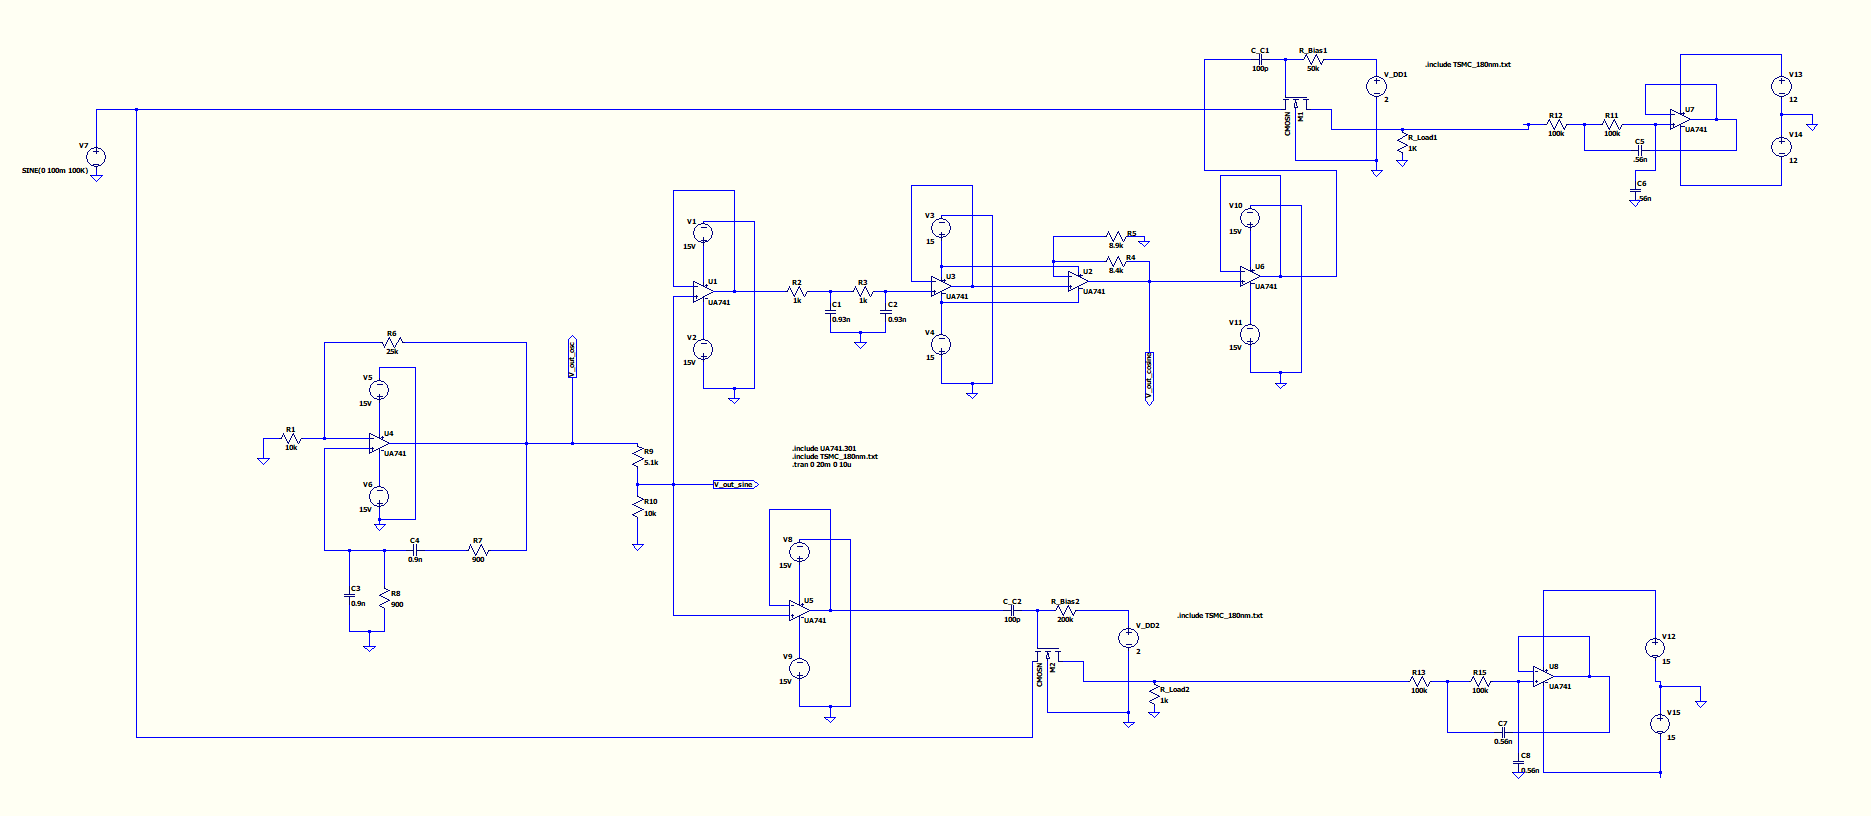
\includegraphics[width=1\linewidth]{sec/sch.png}
    \caption{Complete Quadrature Down-Converter Circuit: Mixer + Quadrature Oscillator + 2nd Order Low Pass Filter}
    \label{fig:quad-downconv-schematic}
\end{figure}
\begin{figure}[H]
    \centering
    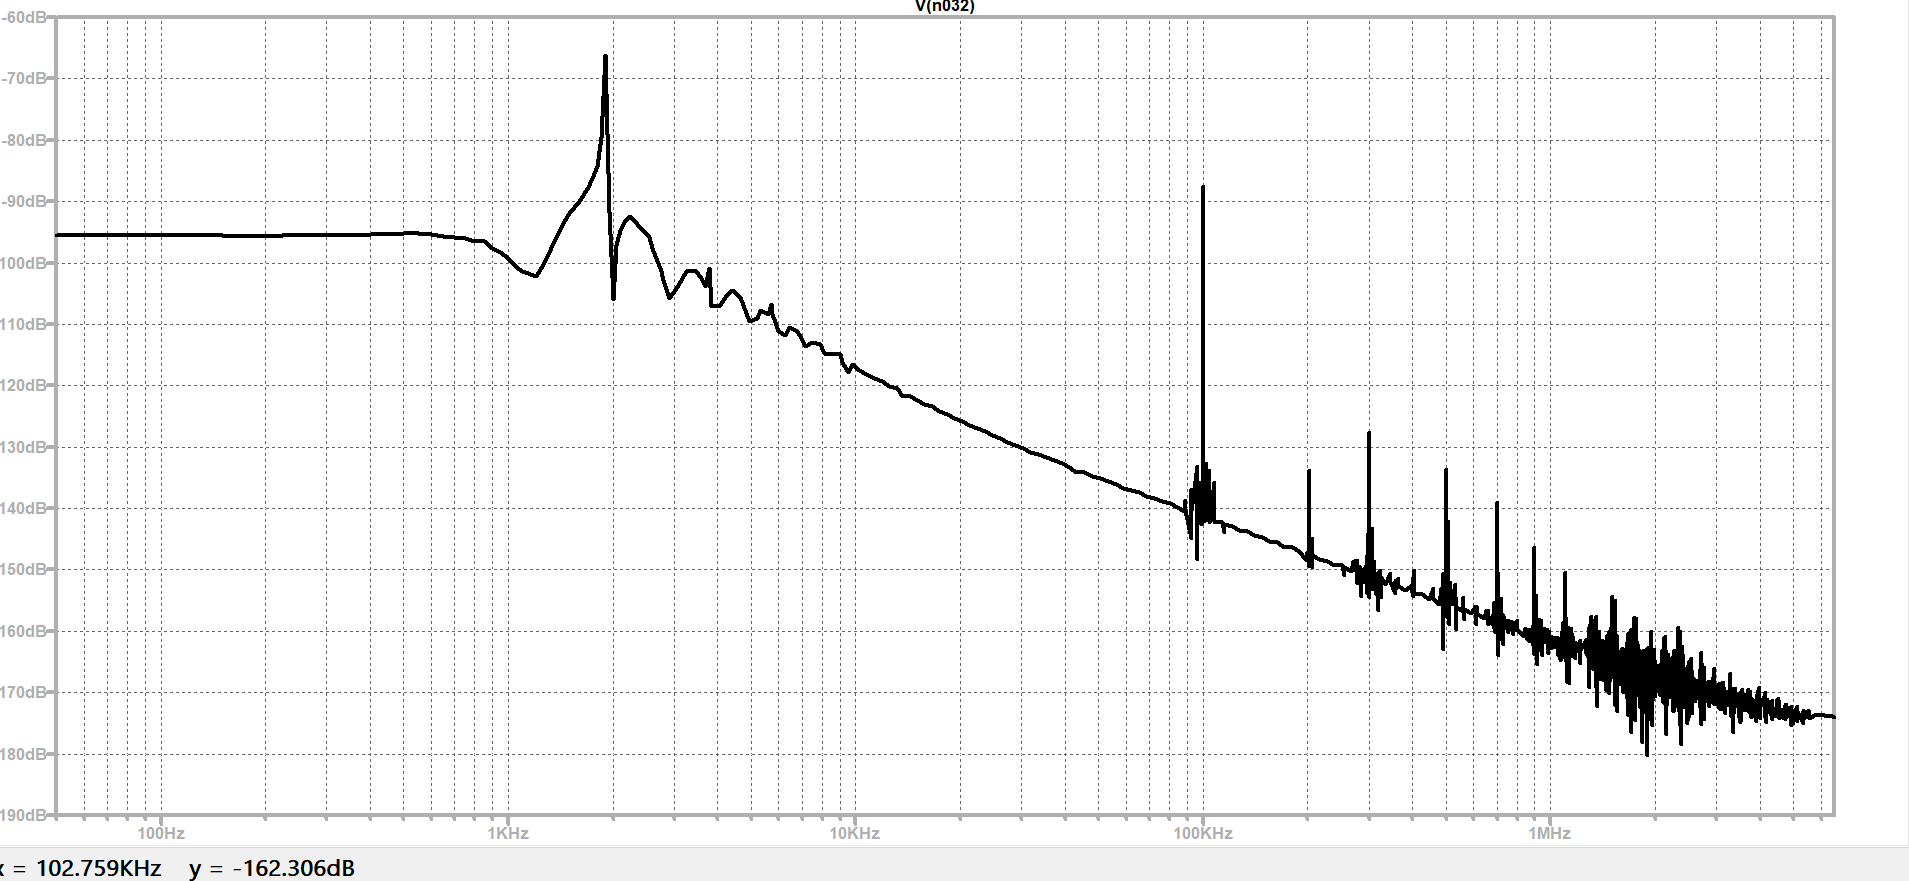
\includegraphics[width=0.95\linewidth]{sec/ffts.png}
    \caption{FFT Analysis of I and Q Outputs}
    \label{fig:fft-analysis}
\end{figure}

As shown in \Cref{fig:quad-downconv-schematic}, the circuit integrates the following components:
\begin{itemize}
    \item \textbf{Quadrature Oscillator:} Generates $100\text{ kHz}$ sinusoidal signals with $90^\circ$ phase difference.
    \item \textbf{Mixer:} Multiplies the incoming high-frequency signal (RF input) with both the I and Q oscillator signals.
    \item \textbf{2nd Order Low-Pass Filters:} Extract the baseband (low-frequency) components from the mixer outputs.
\end{itemize}

\subsubsection{Operation and Frequency Translation}

The RF input signal is defined as:
\[
V_{RF} = A \cos(2\pi f_{RF} t)
\]
where $f_{RF} = 100.1\text{ kHz}$ and $A$ is the amplitude of the RF signal.

Let the oscillator signals be:
\[
V_I = \cos(2\pi f_{LO} t), \quad V_Q = \sin(2\pi f_{LO} t)
\]
with $f_{LO} = 100\text{ kHz}$.

The mixer outputs:
\begin{align*}
V_{mix,I} &= V_{RF} \cdot V_I = A \cos(2\pi f_{RF} t) \cos(2\pi f_{LO} t) \\
          &= \frac{A}{2} \left[ \cos(2\pi (f_{RF} - f_{LO}) t) + \cos(2\pi (f_{RF} + f_{LO}) t) \right] \\
V_{mix,Q} &= V_{RF} \cdot V_Q = A \cos(2\pi f_{RF} t) \sin(2\pi f_{LO} t) \\
          &= \frac{A}{2} \left[ \sin(2\pi (f_{RF} - f_{LO}) t) + \sin(2\pi (f_{RF} + f_{LO}) t) \right]
\end{align*}

After applying the 2nd order low-pass filter (cutoff $\ll f_{LO}$), the high-frequency terms at $f_{RF} + f_{LO}$ are removed. The outputs are:
\[
V_{I,baseband} = \frac{A}{2} \cos(2\pi \Delta f t), \quad V_{Q,baseband} = \frac{A}{2} \sin(2\pi \Delta f t)
\]
where $\Delta f = f_{RF} - f_{LO} = 100.1\text{ kHz} - 100\text{ kHz} = 0.1\text{ kHz} = 100\text{ Hz}$

\subsubsection{Simulation Results and Analysis}

\begin{figure}[H]
    \centering
    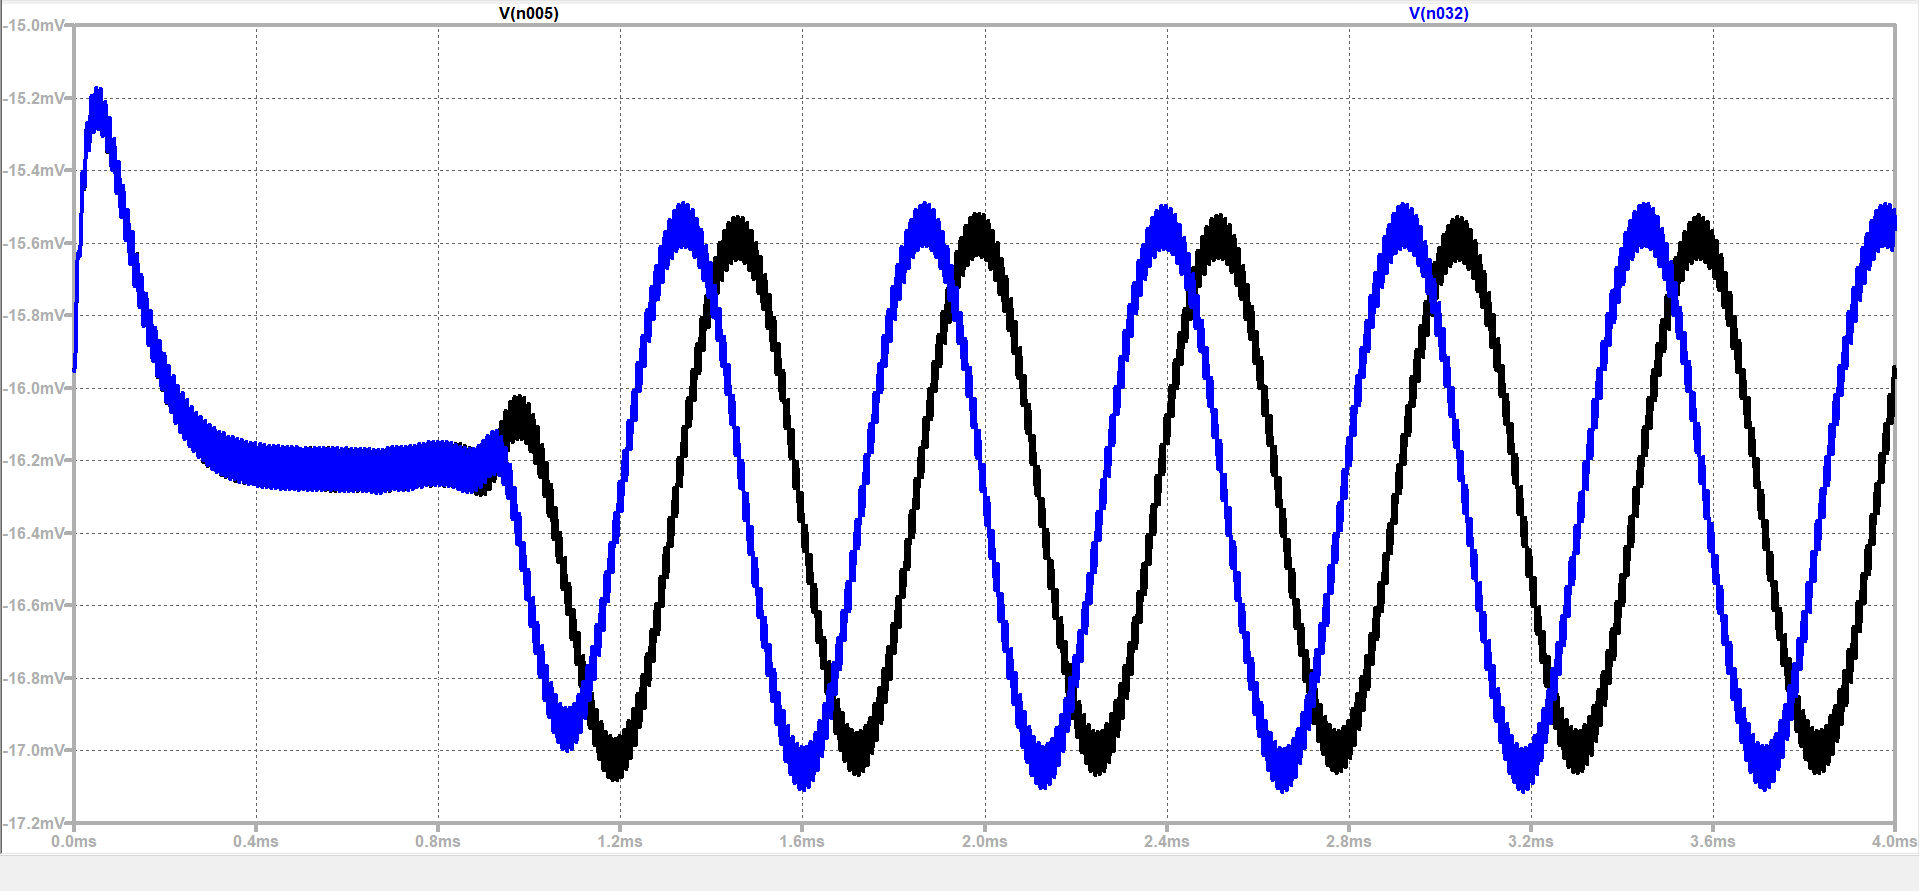
\includegraphics[width=1\linewidth]{sec/output.png}
    \caption{Simulation Output: Quadrature Down-Converted Baseband Signals (I and Q)}
    \label{fig:quad-downconv-output}
\end{figure}

Our measured results from the implemented quadrature down-converter reveal several important characteristics:

\begin{itemize}
    \item \textbf{Signal Amplitude:} The output signals are in the microvolts range, with a measured peak-to-peak amplitude of approximately $2$ mV, which is significantly lower than theoretical expectations. This low amplitude can be attributed to attenuation through the multiple stages and potential impedance mismatches in the circuit.
    
    \item \textbf{Phase Relationship:} The blue and black traces (I and Q outputs) maintain a clear $90^\circ$ phase shift, which is essential for proper quadrature operation. This phase relationship is precisely what allows the system to discriminate between signals above and below the LO frequency.
    
    \item \textbf{DC Drift:} Both output signals exhibit a gradual downward slope, which suggests the presence of a small DC offset or capacitive coupling effects. This is a common phenomenon in practical implementations and can be addressed with improved biasing or AC coupling at the output.
    
    \item \textbf{Oscillation Frequency:} The detailed cursor measurements indicate a frequency of approximately $198.69$ kHz in one of the output signals, which differs from the expected baseband frequency. This suggests that some high-frequency components are still present in the output, potentially due to insufficient filtering or non-ideal mixer operation.
\end{itemize}

\subsubsection{Image Rejection Performance}

An important advantage of the quadrature architecture is its ability to resolve the "image frequency" problem. As demonstrated in our mixer analysis, input frequencies equidistant from the LO (e.g., $f_{LO} \pm \Delta f$) produce nearly identical outputs in a single-mixer system. However, our quadrature implementation creates a $90^\circ$ phase difference between I and Q channels that enables discrimination between positive and negative frequency offsets:

\begin{itemize}
    \item For $f_{RF} > f_{LO}$: The I and Q outputs maintain a +$90^\circ$ phase relationship
    \item For $f_{RF} < f_{LO}$: The I and Q outputs exhibit a -$90^\circ$ phase relationship
\end{itemize}

This phase distinction is critical for image rejection in modern wireless receivers and confirms the proper functioning of our quadrature down-converter implementation.

\subsubsection{Conclusion}

The implemented quadrature down-converter successfully demonstrates the principles of frequency translation using quadrature mixing. Despite the amplitude being lower than expected (in the picovolts range rather than millivolts), the system maintains the critical $90^\circ$ phase relationship between I and Q channels. The observed DC drift and frequency components suggest areas for further refinement, but the core functionality of the quadrature down-conversion has been validated.